<<The root problem with conventional currency is all the trust that's required to make it work. The central bank must be trusted not to debase the currency, but the history of fiat currencies is full of breaches of that trust. Banks must be trusted to hold our money and transfer it electronically, but they lend it out in waves of credit bubbles with barely a fraction in reserve.>> \cite{thebookofsatoshi}\\\\
Beginning with the words of its creator, the pseudonym Satoshi Nakamoto, Bitcoin was born out of a desire to create a decentralized, secure, and accessible form of currency that does not rely on any form of trust in centralized institutions. Bitcoin provides an alternative to conventional currencies and aims to offer greater financial sovereignty to individuals while addressing some of the perceived weaknesses of the existing financial system. Besides that, Bitcoin is a digital currency ecosystem which incorporates many concepts and technologies discovered in the last 50 years of deep research and development around Cryptography, Internet protocol, and Peer-to-Peer networks. It operates through the use of units of currency called "bitcoin" (with a lowercase 'b'), which are used to store and transfer value among participants within the Bitcoin network.\\
Bitcoin protocol enables users to transfer bitcoin across the network, facilitating activities such as buying and selling goods, or sending money to individuals and organizations. Specialized currency exchanges allow for the purchase, sale, and exchange of bitcoin with other fiat currencies. Bitcoin's characteristics make it the perfect type of money for Internet as it offers speed, security, and borderless transactions. Since bitcoin are a form of virtual currencies, the coins are represented in transactions that transfer value from the sender to the recipient. Bitcoin users possess \textbf{private keys} that prove ownership of bitcoin within the Bitcoin network. These keys enable them to sign transactions, unlocking the value and transferring it to a new owner. As already said, Bitcoin is as a \textbf{distributed} peer-to-peer system, who lives without the need for a central server or entity. The creation of new bitcoins is managed through a process called \textbf{mining}. Miners compete to solve mathematical problems while processing Bitcoin transactions. Approximately every 10 minutes, a miner successfully confirms the transactions received from its own node, mining them into a new block, and is rewarded with newly minted bitcoin, called block subsidy. Basically, when miners solve the \textbf{Proof-of-Work} algorithm on the block they are working on, they immediately communicate this new valid block of transactions to all the other Bitcoin nodes which are connected to. At this point, these latter verify the validity of the mined block, and simply add it to their local copy of the ledger shared by every node of the network, the so-called blockchain.\\
The Bitcoin protocol incorporates built-in algorithms that regulate the mining process across the network, such as the \textbf{difficulty adjustment}. The difficulty of the mining activity is dynamically adjusted to ensure that, on average, a miner succeeds every 10 minutes, regardless of the number of miners competing at any given moment. Additionally, the protocol halves the rate at which new bitcoin is created every 4 years (more precisely every 210.000 blocks), and there is a fixed maximum limit of just under \textbf{21 million} coins. Every coin is composed by \textbf{$10^8$ satoshi}, which is the unit of account of the Bitcoin network. By protocol rules, there will be 32 \textbf{halvings}, one every 210.000 blocks. In 2009, the system rewarded successful miners with 50 bitcoin every 10 minutes. The entire emission of bitcoin units can be represented by the following formula:
\[ \sum_{i=0}^{\ 32} 210.000\cdot\frac{50}{2^{i}} \]
Consequently, the number of bitcoins in circulation follows a predictable curve that approaches 21 million by the year 2140. 
\begin{figure}[ht]
\centering
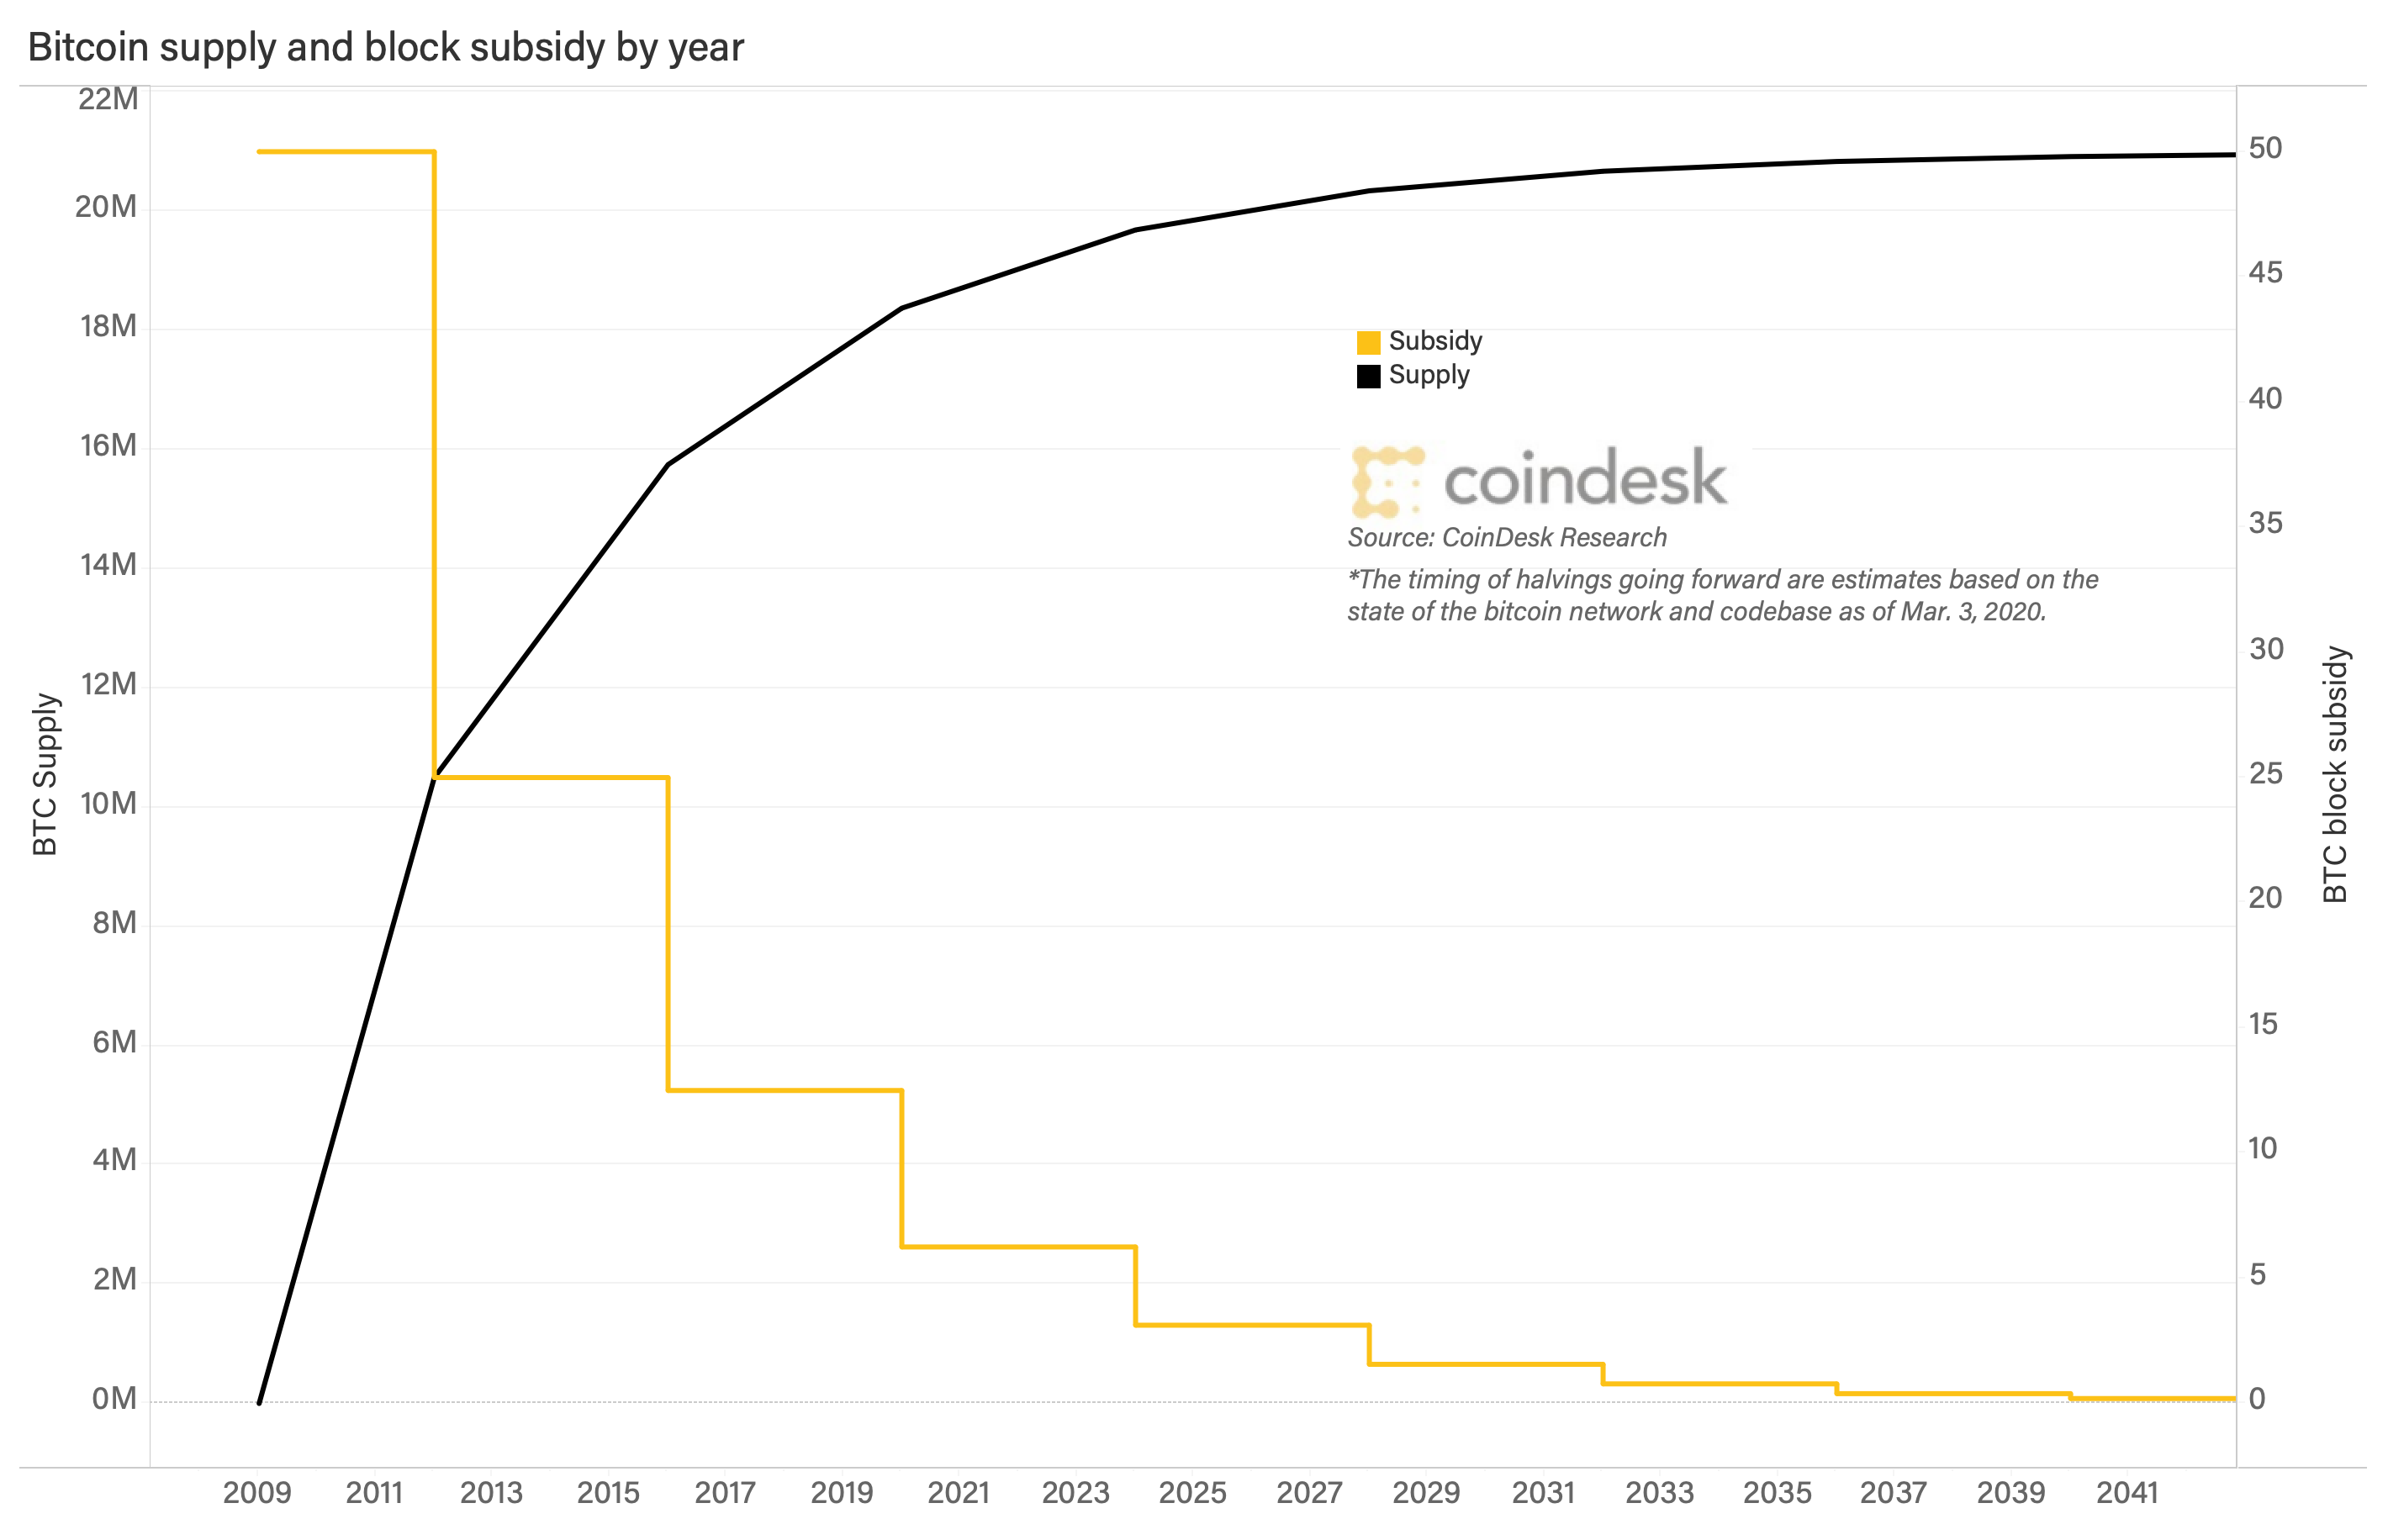
\includegraphics[width=13cm]{Figures/bitcoin/supply_subsidy.png}
\caption{Bitcoin supply and subsidy, \textit{created by Coindesk Research}}
\label{fig:bitcoin_supply}
\end{figure}
\newline\\
As greatly represented in Figure \ref{fig:bitcoin_prehistory}, <<Bitcoin represents the culmination of decades of research in cryptography and distributed systems and includes four key innovations brought together in a unique and powerful combination. Bitcoin consists of:
\begin{itemize}
    \item A decentralized peer-to-peer network (the Bitcoin protocol)
    \item A public transaction ledger (the blockchain)
    \item A set of rules for independent transaction validation and currency issuance (consensus rules)
    \item A mechanism for reaching global decentralized consensus on the valid blockchain (Proof-of-Work algorithm)>> \cite{masteringbitcoin}
\end{itemize}
\noindent In fact, during the late 1980s, with the increasing understanding and availability of cryptography, researchers started to experiment on utilizing cryptography to construct digital currencies. \cite{thebitcoinlegacyprojectBitcoinLegacy}
\begin{figure}[h!]
\centering
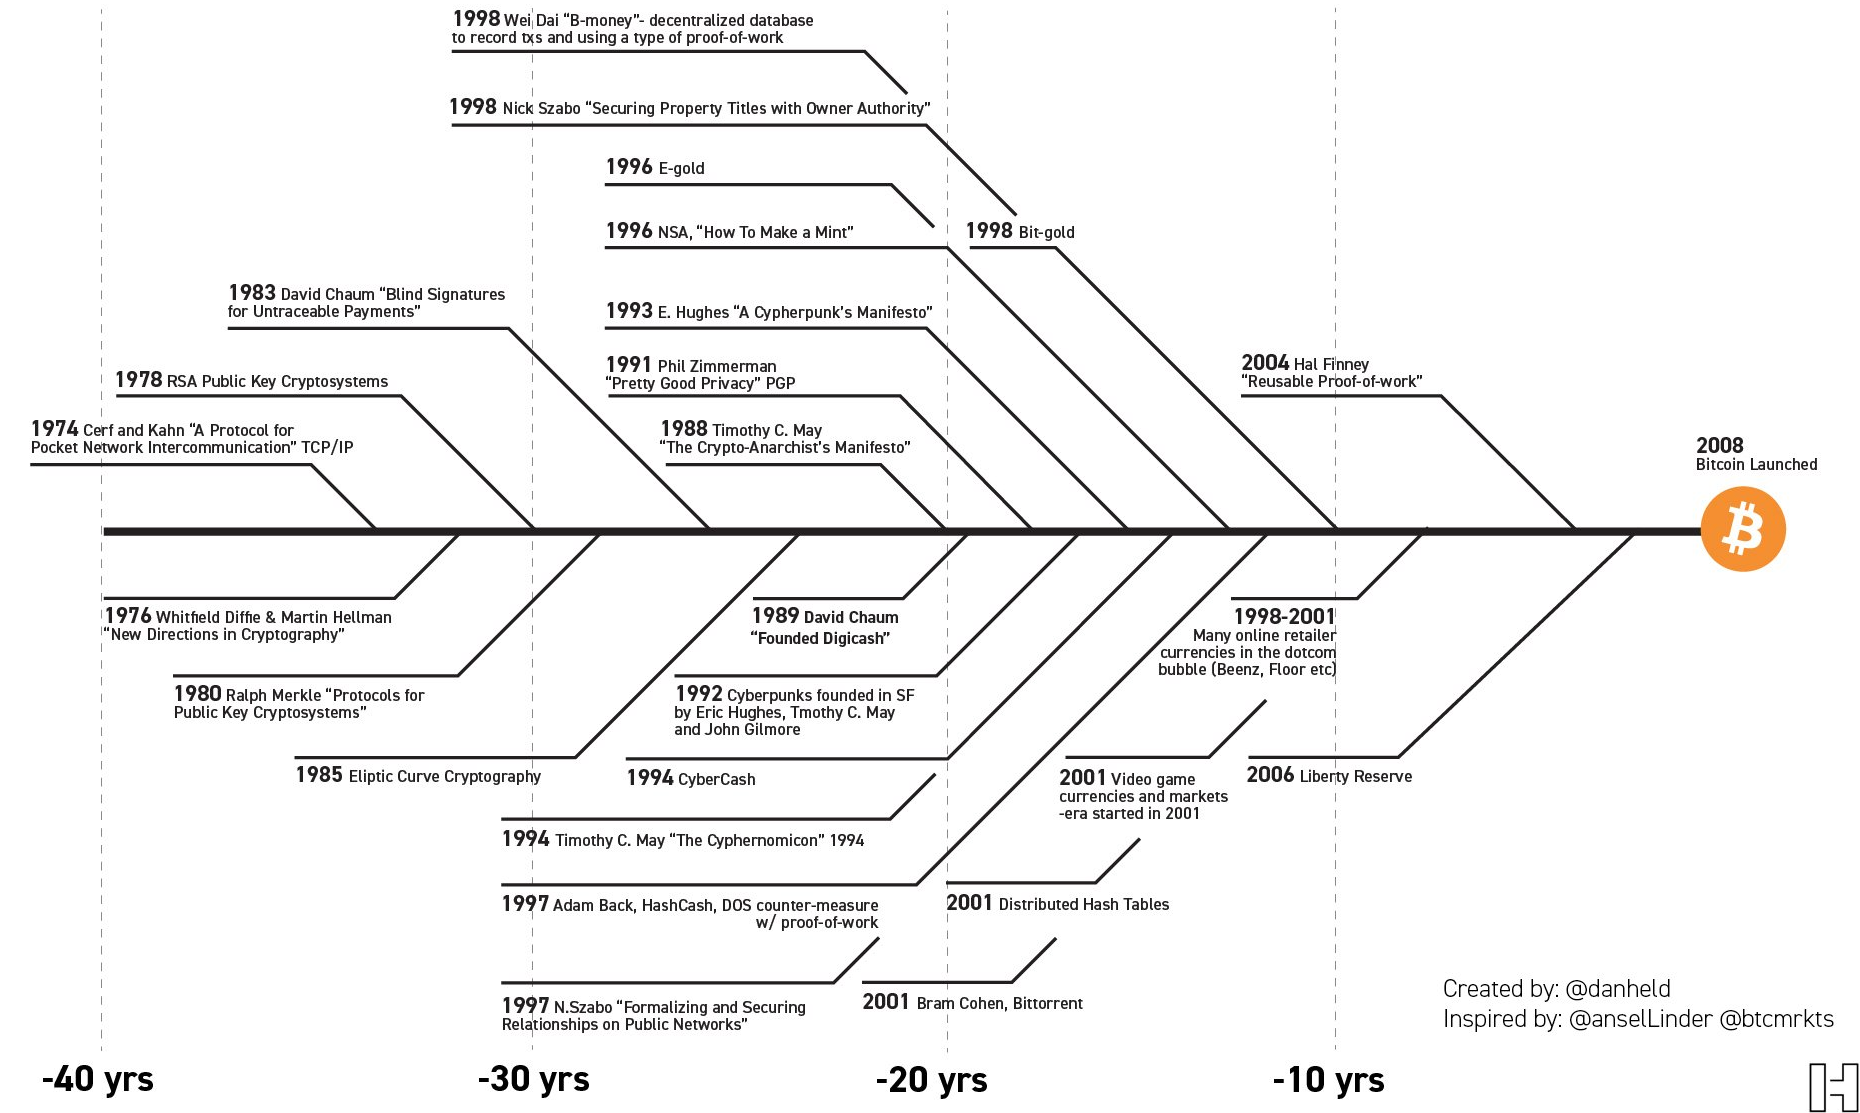
\includegraphics[width=14cm]{Figures/bitcoin/bitcoin-prehistory.png}
\caption{Bitcoin prehistory, \textit{created by @danheld}}
\label{fig:bitcoin_prehistory}
\end{figure}
Valuable examples can be: Ecash (1982, David Chaum), E-gold (1996, Douglas Jackson and Barry Downey), Bit gold (1998, Nick Szabo), B-money (1998, Wei Dai), Reusable Proof of Work (2004, Hal Finney).\\
Even if these initial digital currencies worked effectively, all of them possessed a centralized nature, and for this reason they were susceptible to attacks by governments and malicious hackers.\\\\ \begin{comment}To dig more into the "prehistory" of Bitcoin, it's suggested to have a look at the following link: \href{https://www.thebitcoinlegacyproject.org/}{https://www.thebitcoinlegacyproject.org/}.\end{comment}
    

Finally, on \textbf{3rd of January 2009}, Satoshi Nakamoto created the first block in the Bitcoin blockchain. Since it's the official starting point of the entire Bitcoin history, it's called \textbf{Genesis Block}.\\
In this block, more precisely in the coinbase transaction data, Satoshi left a message which represents the Bitcoin's raison d'\^etre:
\begin{verbatim}
"The Times 03/Jan/2009 Chancellor on brink of second bailout for banks"
\end{verbatim}
This message is a reference to the Times headline of 3rd of January 2009, which proves that the Bitcoin Genesis Block could not have been created before that date. More importantly, the message is a clear statement of the entire Bitcoin movement. It declares the desire to fight the central bank policies, which are characterized by a culture of easy money. Bitcoin, on the other hand, aims to bring back individual responsibility through a monetary system based on sound money. Bitcoin aims to be money which can't be devalued or controlled to benefit a lucky few. 
\begin{figure}[h!]
    \begin{minipage}[t]{0.55\textwidth}
    \centering
    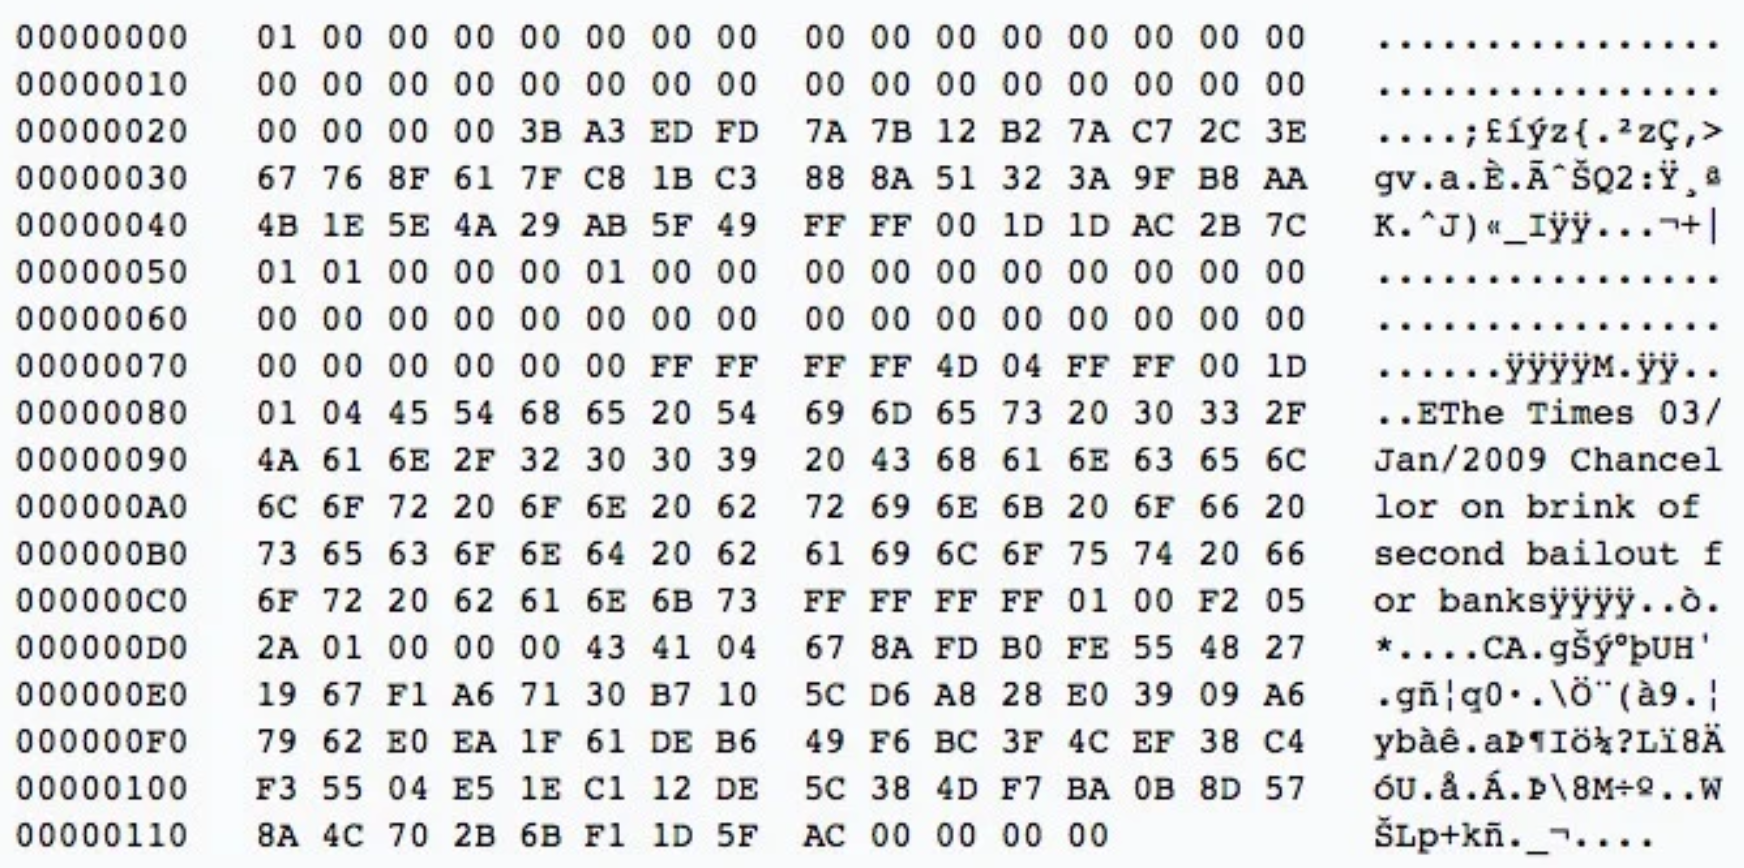
\includegraphics[width=1.1\textwidth]{Figures/bitcoin/genesis-block.png}
    \caption{Bitcoin Genesis Block, \textit{in HEX and ASCII encoding}}
    \label{fig:genesis-block}
    \end{minipage}\hfill
    \begin{minipage}[t]{0.35\textwidth}
    \centering
    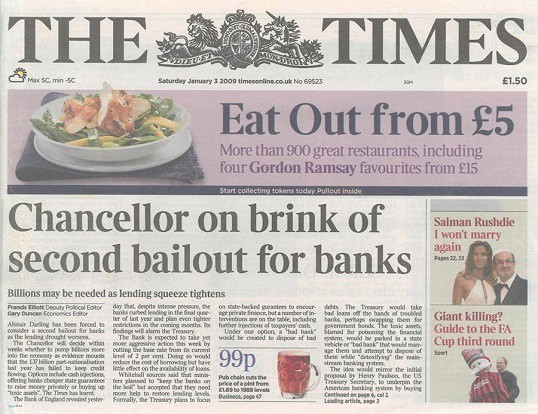
\includegraphics[width=1.1\textwidth]{Figures/bitcoin/times.jpg}
    \caption{Times headline, \textit{Jan 3, 2009}}
    \label{fig:times-headline}
    \end{minipage}
\end{figure}
